\documentclass{standalone}
\usepackage{tikz}
\usetikzlibrary{patterns, positioning}


\begin{document}
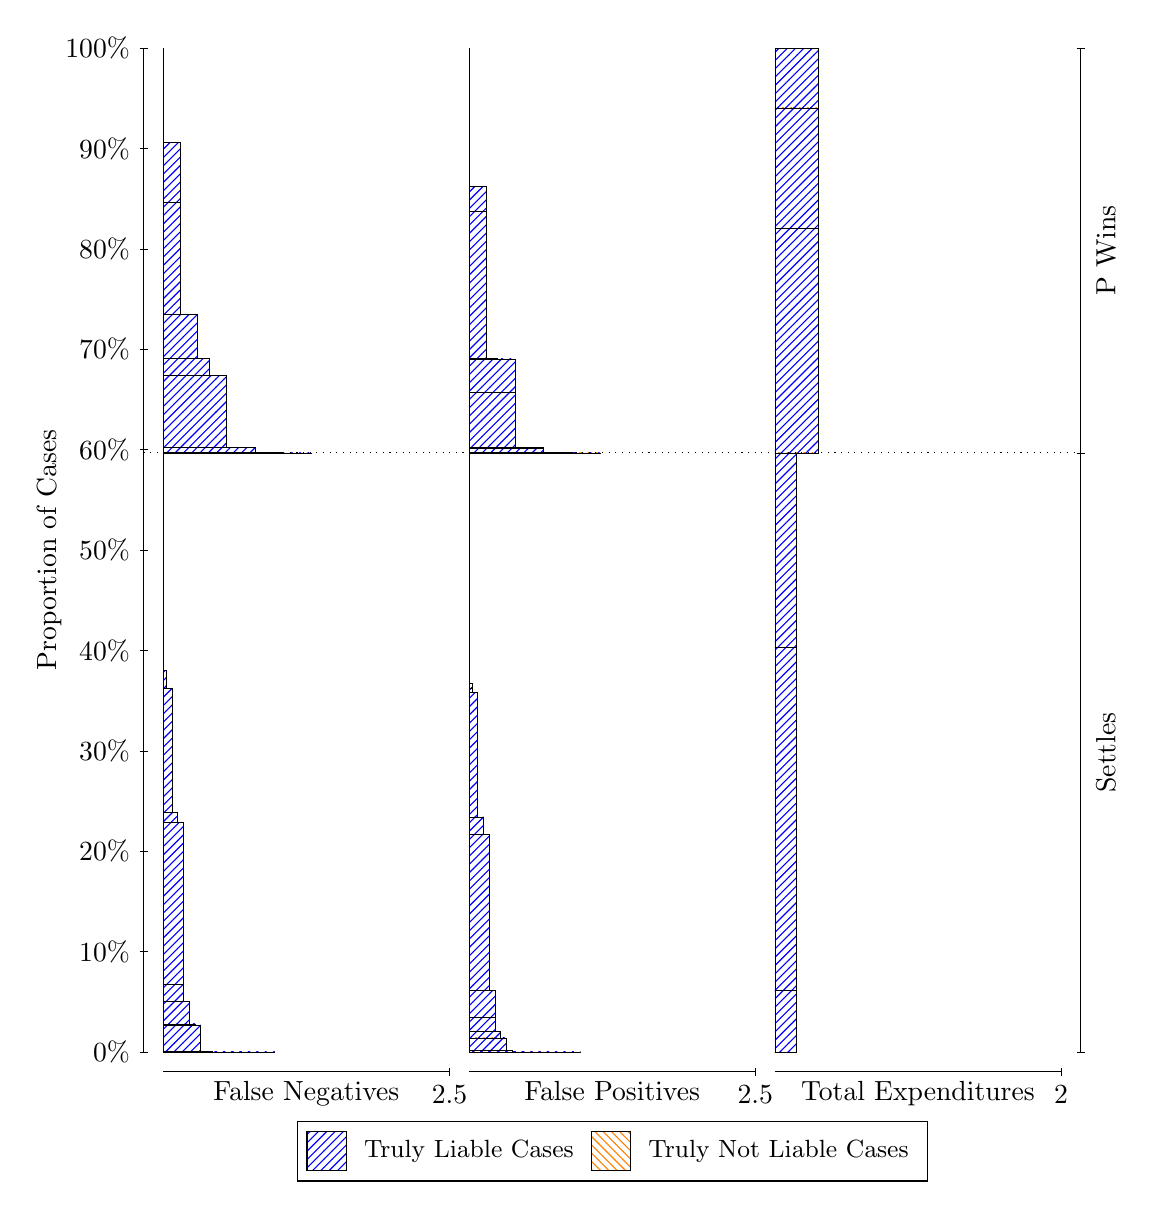
\begin{tikzpicture}
\draw[black, very thin] (1.5,1.75) -- (1.5,14.5);
\node[rotate=90, text=black, anchor=center] at (0.3, 8.125) {Proportion of Cases};
\draw[black, very thin] (1.45,1.75) -- (1.55,1.75);
\node[text=black, anchor=east] at (1.45, 1.75) {0\%};
\draw[black, very thin] (1.45,3.025) -- (1.55,3.025);
\node[text=black, anchor=east] at (1.45, 3.025) {10\%};
\draw[black, very thin] (1.45,4.3) -- (1.55,4.3);
\node[text=black, anchor=east] at (1.45, 4.3) {20\%};
\draw[black, very thin] (1.45,5.575) -- (1.55,5.575);
\node[text=black, anchor=east] at (1.45, 5.575) {30\%};
\draw[black, very thin] (1.45,6.85) -- (1.55,6.85);
\node[text=black, anchor=east] at (1.45, 6.85) {40\%};
\draw[black, very thin] (1.45,8.125) -- (1.55,8.125);
\node[text=black, anchor=east] at (1.45, 8.125) {50\%};
\draw[black, very thin] (1.45,9.4) -- (1.55,9.4);
\node[text=black, anchor=east] at (1.45, 9.4) {60\%};
\draw[black, very thin] (1.45,10.675) -- (1.55,10.675);
\node[text=black, anchor=east] at (1.45, 10.675) {70\%};
\draw[black, very thin] (1.45,11.95) -- (1.55,11.95);
\node[text=black, anchor=east] at (1.45, 11.95) {80\%};
\draw[black, very thin] (1.45,13.225) -- (1.55,13.225);
\node[text=black, anchor=east] at (1.45, 13.225) {90\%};
\draw[black, very thin] (1.45,14.5) -- (1.55,14.5);
\node[text=black, anchor=east] at (1.45, 14.5) {100\%};

\draw[black, very thin] (13.4,1.75) -- (13.4,14.5);
\draw[black, very thin] (13.35,1.75) -- (13.45,1.75);
\node[anchor=west] at (13.35, 1.75) {};
\draw[black, very thin] (13.35,9.3588) -- (13.45,9.3588);
\node[anchor=west] at (13.35, 9.3588) {};
\draw[black, very thin] (13.35,14.5) -- (13.45,14.5);
\node[anchor=west] at (13.35, 14.5) {};

\draw[black, very thin, pattern color=blue, pattern=north east lines] (1.75,1.75) rectangle (3.167,1.75);
\draw[black, very thin, pattern color=blue, pattern=north east lines] (1.75,1.75) rectangle (3.0217,1.75);
\draw[black, very thin, pattern color=blue, pattern=north east lines] (1.75,1.75) rectangle (2.8763,1.75);
\draw[black, very thin, pattern color=blue, pattern=north east lines] (1.75,1.75) rectangle (2.8037,1.75);
\draw[black, very thin, pattern color=blue, pattern=north east lines] (1.75,1.75) rectangle (2.731,1.75);
\draw[black, very thin, pattern color=blue, pattern=north east lines] (1.75,1.75) rectangle (2.6583,1.75);
\draw[black, very thin, pattern color=blue, pattern=north east lines] (1.75,1.75) rectangle (2.5857,1.7508);
\draw[black, very thin, pattern color=blue, pattern=north east lines] (1.75,1.7508) rectangle (2.513,1.7508);
\draw[black, very thin, pattern color=blue, pattern=north east lines] (1.75,1.7508) rectangle (2.4403,1.7512);
\draw[black, very thin, pattern color=blue, pattern=north east lines] (1.75,1.7512) rectangle (2.3677,1.7531);
\draw[black, very thin, pattern color=blue, pattern=north east lines] (1.75,1.7531) rectangle (2.295,1.7565);
\draw[black, very thin, pattern color=blue, pattern=north east lines] (1.75,1.7565) rectangle (2.2223,2.0954);
\draw[black, very thin, pattern color=blue, pattern=north east lines] (1.75,2.0954) rectangle (2.1497,2.1066);
\draw[black, very thin, pattern color=blue, pattern=north east lines] (1.75,2.1066) rectangle (2.077,2.3883);
\draw[black, very thin, pattern color=blue, pattern=north east lines] (1.75,2.3883) rectangle (2.0043,2.6048);
\draw[black, very thin, pattern color=blue, pattern=north east lines] (1.75,2.6048) rectangle (2.0043,4.6706);
\draw[black, very thin, pattern color=blue, pattern=north east lines] (1.75,4.6706) rectangle (1.9317,4.7906);
\draw[black, very thin, pattern color=blue, pattern=north east lines] (1.75,4.7906) rectangle (1.859,6.3734);
\draw[black, very thin, pattern color=blue, pattern=north east lines] (1.75,6.3734) rectangle (1.7863,6.595);
\draw[black, very thin, pattern color=orange, pattern=north west lines] (1.75,6.595) rectangle (1.75,6.595);
\draw[black, very thin, pattern color=blue, pattern=north east lines] (1.75,6.595) rectangle (1.75,9.3588);
\draw[black, very thin, pattern color=blue, pattern=north east lines] (1.75,9.3588) rectangle (3.6393,9.3588);
\draw[black, very thin, pattern color=blue, pattern=north east lines] (1.75,9.3588) rectangle (3.276,9.3598);
\draw[black, very thin, pattern color=blue, pattern=north east lines] (1.75,9.3598) rectangle (3.058,9.3598);
\draw[black, very thin, pattern color=blue, pattern=north east lines] (1.75,9.3598) rectangle (2.9127,9.4318);
\draw[black, very thin, pattern color=blue, pattern=north east lines] (1.75,9.4318) rectangle (2.6947,9.4319);
\draw[black, very thin, pattern color=blue, pattern=north east lines] (1.75,9.4319) rectangle (2.5493,10.339);
\draw[black, very thin, pattern color=blue, pattern=north east lines] (1.75,10.339) rectangle (2.3313,10.561);
\draw[black, very thin, pattern color=blue, pattern=north east lines] (1.75,10.561) rectangle (2.186,11.113);
\draw[black, very thin, pattern color=blue, pattern=north east lines] (1.75,11.113) rectangle (1.968,12.543);
\draw[black, very thin, pattern color=blue, pattern=north east lines] (1.75,12.543) rectangle (1.968,13.305);
\draw[black, very thin, pattern color=blue, pattern=north east lines] (1.75,13.305) rectangle (1.8227,13.307);
\draw[black, very thin, pattern color=orange, pattern=north west lines] (1.75,13.307) rectangle (1.75,13.307);
\draw[black, very thin, pattern color=blue, pattern=north east lines] (1.75,13.307) rectangle (1.75,14.5);
\draw[black, very thin, pattern color=orange, pattern=north west lines] (5.6333,1.75) rectangle (7.0503,1.75);
\draw[black, very thin, pattern color=blue, pattern=north east lines] (5.6333,1.75) rectangle (7.0503,1.75);
\draw[black, very thin, pattern color=orange, pattern=north west lines] (5.6333,1.75) rectangle (6.7597,1.75);
\draw[black, very thin, pattern color=blue, pattern=north east lines] (5.6333,1.75) rectangle (6.7597,1.75);
\draw[black, very thin, pattern color=blue, pattern=north east lines] (5.6333,1.75) rectangle (6.687,1.75);
\draw[black, very thin, pattern color=orange, pattern=north west lines] (5.6333,1.75) rectangle (6.6143,1.75);
\draw[black, very thin, pattern color=blue, pattern=north east lines] (5.6333,1.75) rectangle (6.6143,1.75);
\draw[black, very thin, pattern color=orange, pattern=north west lines] (5.6333,1.75) rectangle (6.469,1.75);
\draw[black, very thin, pattern color=blue, pattern=north east lines] (5.6333,1.75) rectangle (6.469,1.7503);
\draw[black, very thin, pattern color=blue, pattern=north east lines] (5.6333,1.7503) rectangle (6.3963,1.7503);
\draw[black, very thin, pattern color=orange, pattern=north west lines] (5.6333,1.7503) rectangle (6.3237,1.7503);
\draw[black, very thin, pattern color=blue, pattern=north east lines] (5.6333,1.7503) rectangle (6.3237,1.7508);
\draw[black, very thin, pattern color=blue, pattern=north east lines] (5.6333,1.7508) rectangle (6.3237,1.7513);
\draw[black, very thin, pattern color=blue, pattern=north east lines] (5.6333,1.7513) rectangle (6.251,1.7513);
\draw[black, very thin, pattern color=orange, pattern=north west lines] (5.6333,1.7513) rectangle (6.1783,1.7513);
\draw[black, very thin, pattern color=blue, pattern=north east lines] (5.6333,1.7513) rectangle (6.1783,1.7664);
\draw[black, very thin, pattern color=blue, pattern=north east lines] (5.6333,1.7664) rectangle (6.1057,1.9292);
\draw[black, very thin, pattern color=orange, pattern=north west lines] (5.6333,1.9292) rectangle (6.033,1.9292);
\draw[black, very thin, pattern color=blue, pattern=north east lines] (5.6333,1.9292) rectangle (6.033,2.0089);
\draw[black, very thin, pattern color=blue, pattern=north east lines] (5.6333,2.0089) rectangle (6.033,2.0115);
\draw[black, very thin, pattern color=blue, pattern=north east lines] (5.6333,2.0115) rectangle (5.9603,2.1895);
\draw[black, very thin, pattern color=blue, pattern=north east lines] (5.6333,2.1895) rectangle (5.9603,2.5273);
\draw[black, very thin, pattern color=orange, pattern=north west lines] (5.6333,2.5273) rectangle (5.8877,2.5273);
\draw[black, very thin, pattern color=blue, pattern=north east lines] (5.6333,2.5273) rectangle (5.8877,4.5134);
\draw[black, very thin, pattern color=blue, pattern=north east lines] (5.6333,4.5134) rectangle (5.8877,4.5138);
\draw[black, very thin, pattern color=blue, pattern=north east lines] (5.6333,4.5138) rectangle (5.815,4.7354);
\draw[black, very thin, pattern color=blue, pattern=north east lines] (5.6333,4.7354) rectangle (5.7423,6.3181);
\draw[black, very thin, pattern color=blue, pattern=north east lines] (5.6333,6.3181) rectangle (5.6697,6.3747);
\draw[black, very thin, pattern color=blue, pattern=north east lines] (5.6333,6.3747) rectangle (5.6697,6.4382);
\draw[black, very thin, pattern color=blue, pattern=north east lines] (5.6333,6.4382) rectangle (5.6333,9.3588);
\draw[black, very thin, pattern color=orange, pattern=north west lines] (5.6333,9.3588) rectangle (7.3047,9.3588);
\draw[black, very thin, pattern color=blue, pattern=north east lines] (5.6333,9.3588) rectangle (7.3047,9.3588);
\draw[black, very thin, pattern color=orange, pattern=north west lines] (5.6333,9.3588) rectangle (6.9413,9.3588);
\draw[black, very thin, pattern color=blue, pattern=north east lines] (5.6333,9.3588) rectangle (6.9413,9.359);
\draw[black, very thin, pattern color=blue, pattern=north east lines] (5.6333,9.359) rectangle (6.9413,9.3598);
\draw[black, very thin, pattern color=orange, pattern=north west lines] (5.6333,9.3598) rectangle (6.578,9.3598);
\draw[black, very thin, pattern color=blue, pattern=north east lines] (5.6333,9.3598) rectangle (6.578,9.4114);
\draw[black, very thin, pattern color=blue, pattern=north east lines] (5.6333,9.4114) rectangle (6.578,9.4279);
\draw[black, very thin, pattern color=orange, pattern=north west lines] (5.6333,9.4279) rectangle (6.36,9.4279);
\draw[black, very thin, pattern color=blue, pattern=north east lines] (5.6333,9.4279) rectangle (6.36,9.4279);
\draw[black, very thin, pattern color=orange, pattern=north west lines] (5.6333,9.4279) rectangle (6.2147,9.4279);
\draw[black, very thin, pattern color=blue, pattern=north east lines] (5.6333,9.4279) rectangle (6.2147,10.127);
\draw[black, very thin, pattern color=blue, pattern=north east lines] (5.6333,10.127) rectangle (6.2147,10.552);
\draw[black, very thin, pattern color=orange, pattern=north west lines] (5.6333,10.552) rectangle (5.9967,10.552);
\draw[black, very thin, pattern color=blue, pattern=north east lines] (5.6333,10.552) rectangle (5.9967,10.554);
\draw[black, very thin, pattern color=blue, pattern=north east lines] (5.6333,10.554) rectangle (5.8513,12.427);
\draw[black, very thin, pattern color=blue, pattern=north east lines] (5.6333,12.427) rectangle (5.8513,12.745);
\draw[black, very thin, pattern color=orange, pattern=north west lines] (5.6333,12.745) rectangle (5.6333,12.745);
\draw[black, very thin, pattern color=blue, pattern=north east lines] (5.6333,12.745) rectangle (5.6333,14.5);
\draw[black, very thin, pattern color=orange, pattern=north west lines] (9.5167,1.75) rectangle (9.7892,1.75);
\draw[black, very thin, pattern color=blue, pattern=north east lines] (9.5167,1.75) rectangle (9.7892,2.5313);
\draw[black, very thin, pattern color=orange, pattern=north west lines] (9.5167,2.5313) rectangle (9.7892,2.5313);
\draw[black, very thin, pattern color=blue, pattern=north east lines] (9.5167,2.5313) rectangle (9.7892,6.8846);
\draw[black, very thin, pattern color=orange, pattern=north west lines] (9.5167,6.8846) rectangle (9.7892,6.8846);
\draw[black, very thin, pattern color=blue, pattern=north east lines] (9.5167,6.8846) rectangle (9.7892,9.3588);
\draw[black, very thin, pattern color=orange, pattern=north west lines] (9.5167,9.3588) rectangle (10.062,9.3588);
\draw[black, very thin, pattern color=blue, pattern=north east lines] (9.5167,9.3588) rectangle (10.062,12.205);
\draw[black, very thin, pattern color=orange, pattern=north west lines] (9.5167,12.205) rectangle (10.062,12.205);
\draw[black, very thin, pattern color=blue, pattern=north east lines] (9.5167,12.205) rectangle (10.062,13.74);
\draw[black, very thin, pattern color=orange, pattern=north west lines] (9.5167,13.74) rectangle (10.062,13.74);
\draw[black, very thin, pattern color=blue, pattern=north east lines] (9.5167,13.74) rectangle (10.062,14.5);
\draw[black, dotted] (1.5,9.3588) -- (13.4,9.3588);
\draw[black, very thin] (1.75,1.5) -- (5.3833,1.5);
\node[text=black, anchor=north] at (3.5667, 1.5) {False Negatives};
\draw[black, very thin] (5.3833,1.45) -- (5.3833,1.55);
\node[text=black, anchor=north] at (5.3833, 1.45) {2.5};

\draw[black, very thin] (5.6333,1.5) -- (9.2667,1.5);
\node[text=black, anchor=north] at (7.45, 1.5) {False Positives};
\draw[black, very thin] (9.2667,1.45) -- (9.2667,1.55);
\node[text=black, anchor=north] at (9.2667, 1.45) {2.5};

\draw[black, very thin] (9.5167,1.5) -- (13.15,1.5);
\node[text=black, anchor=north] at (11.333, 1.5) {Total Expenditures};
\draw[black, very thin] (13.15,1.45) -- (13.15,1.55);
\node[text=black, anchor=north] at (13.15, 1.45) {2};

\node[text=black, centered, rotate=90] at (13.72, 5.5544) {Settles};
\node[text=black, centered, rotate=90] at (13.72, 11.929) {P Wins};

\draw (7.449999999999999,1.5) node[draw=none] (baseCoordinate) {};
\begin{scope}[align=center]
        \matrix[scale=0.5, draw=black, below=0.5cm of baseCoordinate, nodes={draw}, column sep=0.1cm]{
            \node[rectangle, draw, minimum width=0.5cm, minimum height=0.5cm, pattern color=blue, pattern=north east lines] {}; &
            \node[draw=none, font=\small, text=black] (B) {Truly Liable Cases}; &
            \node[rectangle, draw, minimum width=0.5cm, minimum height=0.5cm, pattern color=orange, pattern=north west lines] {}; &
            \node[draw=none, font=\small, text=black] (B) {Truly Not Liable Cases}; \\
            };
\end{scope}

\end{tikzpicture}
\end{document}